\usetikzlibrary{shapes, arrows.meta, positioning, fit, decorations.pathreplacing,
  decorations.pathmorphing, decorations.shapes, calc}

\pgfdeclarelayer{background}
\pgfdeclarelayer{middle}
\pgfsetlayers{background,middle,main}

\tikzset{dada2/.style={draw, fill=green!10, align=center}}
\tikzset{vsearch/.style={draw, fill=red!20, align=center}}
\tikzset{usearch/.style={draw, fill=magenta!10, align=center}}
\tikzset{cutadapt/.style={draw, fill=cyan!10, align=center}}
\tikzset{protax/.style={draw, fill=blue!15, align=center}}
\tikzset{protax_or_vsearch/.style={draw, shade, right color=blue!15, left color=red!20, align=center}}
\tikzset{protax_or_usearch/.style={draw, shade, right color=blue!15, left color=magenta!10, align=center}}
\tikzset{infernal/.style={draw, fill=orange!15, align=center}}
\tikzset{new/.style={draw, fill=yellow!10, align=center}}
\tikzset{data/.style={align=center}}
\tikzset{key/.style={minimum width=35mm}}

% \tikzset{parallel/.style={dotted, line width=1pt}}
\tikzset{parallel/.style={fill=gray!20, rounded corners}}
\tikzset{paired reads/.style={line width = 1pt, double distance=0.5pt,decorate, decoration={snake, amplitude=0.75pt, segment length = 3pt, post=lineto, post length=2mm}}}
\tikzset{single reads/.style={decorate, decoration={snake, amplitude=0.75pt, segment length = 3pt, post=lineto, post length=2mm}}}
\tikzset{table/.style={line width=1pt}}
\tikzset{taxonomy/.style={double distance=0.5pt}}

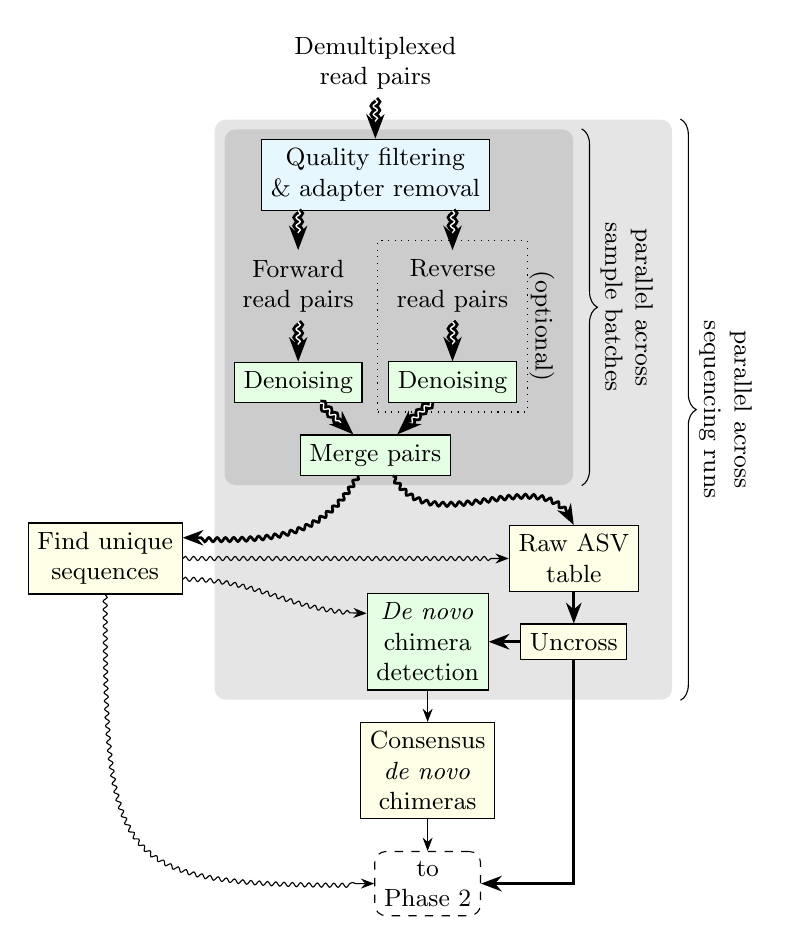
\begin{tikzpicture}[font=\small,node distance=4mm]
\node[data] (raw) {Demultiplexed \\ read pairs};

\node[below=5mm of raw, cutadapt] (filter) {Quality filtering \\ \& adapter removal};
\coordinate[below=5mm of filter] (readcenter);
\node[below left=5mm and 1.5mm of filter.south, data] (fwdreads) {Forward\\read pairs};
\node[below right=5mm and 1.5mm of filter.south, data] (revreads) {Reverse\\read pairs};
\node[below=5mm of fwdreads, dada2] (denoise) {Denoising};
\node[below=5mm of revreads, dada2] (denoiserc) {Denoising};
\node[draw, fit=(revreads) (denoiserc), dotted](rc){};
\node[right=1mm of rc, anchor=base, align=center, rotate=-90] (rev_option) {(optional)};
\node[below=of $(denoise.south)!.5!(denoiserc.south)$, dada2] (merge) {Merge pairs};
\begin{pgfonlayer}{middle}
\node[parallel, fit=(filter) (merge) (denoise) (rev_option), fill=gray!40] (sample_batch) {};
\end{pgfonlayer}
\draw[decorate, decoration={brace, raise = 1mm, amplitude=2mm}] (sample_batch.north east) -- (sample_batch.south east) ;
\node[rotate=-90,right=4mm of sample_batch, anchor=base, align=center] (sample_batch_label) {parallel across \\ sample batches};

\node[below = 5mm of sample_batch.south east, new] (seqtable_raw) {Raw ASV\\table};
\node[below=of seqtable_raw, new] (uncross) {Uncross};
\node[left=of uncross, dada2] (chimera1) {\emph{De novo} \\ chimera \\ detection};
\begin{pgfonlayer}{background}
\node[parallel, fit=(sample_batch) (chimera1) (sample_batch_label) (seqtable_raw)](seqrun){};
\end{pgfonlayer}
\draw[decorate, decoration={brace, raise = 1mm, amplitude=2mm}] (seqrun.north east) -- (seqrun.south east) ;
\node[rotate=-90,right=4mm of seqrun, anchor=base, align=center] {parallel across \\ sequencing runs};

\node[below=of chimera1, new] (combine) {Consensus \\ \emph{de novo} \\ chimeras};

\node[left = of $(seqtable_raw-|seqrun.west)$, new] (seq_all) {Find unique\\sequences};

\node[below=of combine, draw, rounded corners, dashed, align=center] (phase2) {to \\ Phase 2};

\draw[-Stealth,paired reads] (raw) -- (filter);
\draw[-Stealth,paired reads] (fwdreads.north|-filter.south) -- (fwdreads);
\draw[-Stealth,paired reads] (revreads.north|-filter.south) -- (revreads);
\draw[-Stealth,paired reads] (fwdreads) -- (denoise);
\draw[-Stealth,paired reads] (revreads) -- (denoiserc);
\draw[-Stealth,paired reads] (denoise) -- (merge);
\draw[-Stealth,paired reads] (denoiserc) -- (merge);
\draw[-Stealth,single reads,table] (merge.230) .. controls +(240:10mm) and +(0:10mm) .. (seq_all.15);
\draw[-Stealth,single reads,table] (merge.310) .. controls +(300:10mm) and +(110:10mm) .. (seqtable_raw.north);
\draw[-Stealth,single reads] (seq_all) -- (seqtable_raw);
\draw[-Stealth,table] (seqtable_raw) -- (uncross);
\draw[-Stealth,single reads] (seq_all.345) .. controls +(0:10mm) and +(180:10mm) .. (chimera1.155);
\draw[-Stealth,table] (uncross) -- (chimera1);
\draw[-Stealth] (chimera1) -- (combine);
\draw[-Stealth, single reads] (seq_all) .. controls +(270:40mm) and +(180:40mm) .. (phase2);
\draw[-Stealth] (combine) -- (phase2);
\draw[-Stealth, table] (uncross) |- (phase2);
\end{tikzpicture}
